\documentclass{article}

\usepackage[spanish]{babel}
\usepackage[numbers,sort&compress]{natbib}
\usepackage{graphicx}
\usepackage{url}
\usepackage{amsmath}
\usepackage{hyperref}
\usepackage[top=30mm, bottom=40mm, left=15mm, right=15mm]{geometry}
\usepackage{listings}
\usepackage{subfig}
\usepackage{color}
\usepackage{multirow}
\usepackage[latin1]{inputenc}

\setlength{\parskip}{2mm}
\setlength{\parindent}{0pt}
\definecolor{dkgreen}{rgb}{0,0.6,0}
\definecolor{gray}{rgb}{0.3,0.3,0.3}
\definecolor{orange}{rgb}{0.8,0.4,0}
\definecolor{mostaza}{rgb}{0.9,0.8,0.1}

\lstset{ %
  language=R,                     % the language of the code
  basicstyle=\footnotesize,       % the size of the fonts that are used for the code
  numbers=left,                   % where to put the line-numbers
  numberstyle=\tiny\color{gray},  % the style that is used for the line-numbers
  stepnumber=1,                   % the step between two line-numbers. If it's 1, each line
                                  % will be numbered
  numbersep=5pt,                  % how far the line-numbers are from the code
  backgroundcolor=\color{white},  % choose the background color. You must add \usepackage{color}
  showspaces=false,               % show spaces adding particular underscores
  showstringspaces=false,         % underline spaces within strings
  showtabs=false,                 % show tabs within strings adding particular underscores
  frame=single,                   % adds a frame around the code
  rulecolor=\color{black},        % if not set, the frame-color may be changed on line-breaks within not-black text (e.g. commens (green here))
  tabsize=2,                      % sets default tabsize to 2 spaces
  captionpos=b,                   % sets the caption-position to bottom
  breaklines=true,                % sets automatic line breaking
  breakatwhitespace=false,        % sets if automatic breaks should only happen at whitespace
  title=\lstname,                 % show the filename of files included with \lstinputlisting;
                                  % also try caption instead of title
  keywordstyle=\color{orange},      % keyword style
  commentstyle=\color{dkgreen},   % comment style
  stringstyle=\color{mostaza},      % string literal style
  escapeinside={\%*}{*)},         % if you want to add a comment within your code
  morekeywords={*,...}            % if you want to add more keywords to the set
} 

\author{Marco Antonio Guajardo Vigil  2095}
\title{\textbf{Pr\'actica 7: B\'usqueda local} \\ Simulaci\'on de sistemas}
\date{19 de marzo, 2019}

\begin{document}

\maketitle

\section{Introducci\'on}
En la s\'eptima pr\'actica se implementa una optimizaci\'on huer\'istica sencilla para encontrar m\'aximos locales de funciones.
Se busca m\'aximizar la funci\'on bidimensional $g(x,y)$ \ref{eqn:fxy} :

\begin{equation}
g(x,y) = \frac{(x + 0.5)^4 - 30x^2 - 20x + (y + 0.5)^4 - 30y^2 - 20y}{100}
\label{eqn:fxy},
\end{equation}

a partir de un punto seleccionado al azar, realizando movimientos locales.

\section{Objetivo}

Se maximiza la funci\'on bidimensional, $g(x,y)$, con restricciones $-3 \leq  x,y \leq 3$. La posici\'on actual es un par $x,y$ y se ocupan dos movimientos aleatorios, $\Delta x$ y $\Delta y$, cuyas combinaciones posibles proveen ocho posiciones vecinos, de los cuales aquella que logra el mayor valor para $g$ es seleccionado. Dibujando $g(x,y)$ en tres dimensiones obtenemos la figura \ref{fig:3d}.

Se crea una visualizaci\'on animada de c\'omo proceden \textbf{15} r\'eplicas simut\'aneas de la b\'usqueda encima de una gr\'afica de proyecci\'on plana.

\begin{figure}[h!]
\centering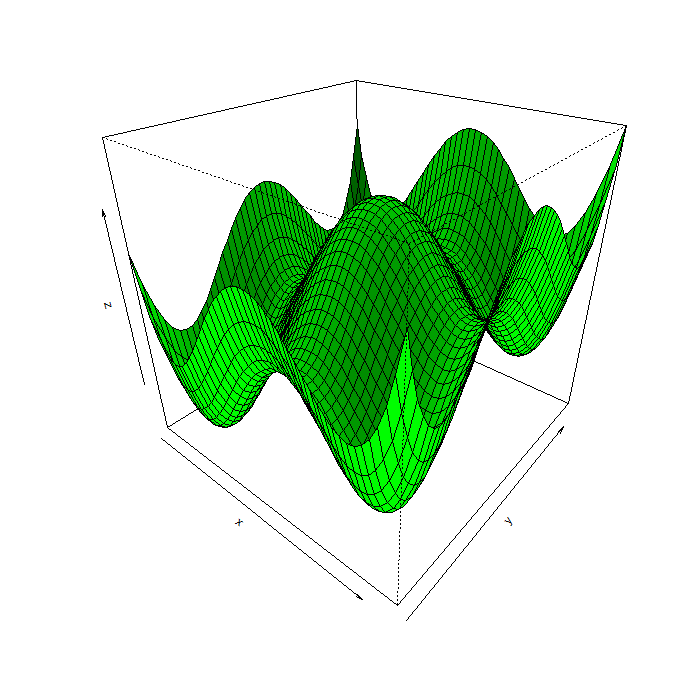
\includegraphics[width=50mm]{3d.png}
\caption{Modelo en tres dimensiones de la funci\'on $g(x,y)$.}
\label{fig:3d}
\end{figure}

\newpage

\subsection{Implementaci\'on de R}
Para la elaboraci\'on de este experimento, se hace uso de un software libre para computaci\'on estad\'istica y gr\'aficos llamado \citet{R}, el cual nos permite realizar los c\'alculos necesarios para dicho experimento. Con \'el, se pueden controlar los datos estad\'isticos que se ocupan para dar seguimiento con la pr\'actica, se necesita graficarlos para as\'i poder compararlos mejor, ya que se maneja una cantidad de datos considerable y trabajaremos con ellos en forma estad\'istica.

\subsection{Experimentaci\'on}

Se crea un \texttt{data.frame()} llamado \texttt{coordenadas}, este almacena la mejor posici\'on $(x,y)$ obtenida entre los ocho vecinos, tambi\'en se almacena el n\'umero de pasos en el cual se obtuvo ese valor, se establecen los l\'imites (\texttt{low} y \texttt{high}) mencionados anteriormente en el objetivo, el punto avanza en pasos de 0.25 declarado en \texttt{step}.

\begin{lstlisting}[language=R]
low <- -3
high <- -low
step <- 0.25
replicas <- 15
coordenadas <- data.frame("X"=0, "Y"=0, "T"=0, "R" = 0)
animacion <- FALSE
\end{lstlisting}

Se modifica el c\'odigo obtenido de la Dr. Elisa Shaeffer \cite{SatuP7} que inicialmente obtenia los m\'inimos de una funci\'on unidimensional, de tal modo que permita encontrar los m\'aximos locales de la funci\'on bidimensional $g(x,y)$, estas modificaciones se presentan en el siguiente c\'odigo:

\begin{lstlisting}[language=R]
replica <- function(t, coor) {
  currX <- runif(1, low, high) 
  currY <- runif(1, low, high)
  bestX <- currX
  bestY <- currY
  for (tiempo in 1:t) {
    deltaX <- runif(1, 0, step)
    deltaY <- runif(1, 0, step)
    izq <- currX - deltaX
    der <- currX + deltaX
    abajo <- currY - deltaY
    arriba <- currY + deltaY
    while(sum(c(izq, der, abajo, arriba) < low) !=0 || sum(c(izq, der, abajo, arriba) > high) != 0){
      currX <- runif(1, low, high) 
      currY <- runif(1, low, high)
      deltaX <- runif(1, 0, step)
      deltaY <- runif(1, 0, step)
      izq <- currX - deltaX
      der <- currX + deltaX
      abajo <- currY - deltaY
      arriba <- currY + deltaY 
     b = data.frame("X" = bestX, "Y" = bestY, "T" = tiempo, "R" = i)
     coor <- rbind(coor, b)
    }
  best = c(bestX, bestY)
  return(coor)
}
\end{lstlisting}

\newpage

Se paralelizan las r\'eplicas para realizarlas simult\'aneamente y se crean figuras en donde se muestran cada una de las r\'eplicas buscando el mayor vecino, hasta llegar a la m\'axima posici\'on.

\begin{lstlisting}[language=R]
suppressMessages(library(doParallel))
registerDoParallel(makeCluster(detectCores() - 1))
values <- seq(low, high, by = step)
x <- rep(values, each = length(values))
y <- rep(values, length(values))
z <- foreach(i = x, j = y, .combine=c) %dopar% g(i,j)
resultados2 <- data.frame(x, y, z)
tmax <- 10^4
resultados <- foreach(i = 1:replicas, .combine="rbind") %dopar% replica(tmax, coordenadas)
resultados <- data.frame(resultados)
stopImplicitCluster()
resultados <- resultados[!(resultados$T == 0),]
library(ggplot2)
for (i in 1:tmax){
  sS <- subset(resultados, T == i)
  if(animacion){
    ggsave(paste("paso", i, ".png", sep=""))
    ggplot(resultados2, aes(x = x, y = y)) + geom_tile(aes(fill=z)) + ggtitle(paste("Paso ", i, sep="")) +
      scale_fill_gradient2(name = "",low = "orange", mid = "yellow", high = "red", midpoint=(min(z)+max(z))/2, breaks = c(seq(floor(min(z)), 0, by = 0.5))) +
      scale_x_continuous("", breaks = seq(low, high, by = 1)) + scale_y_continuous("", breaks = seq(low, high, by = 1)) +
      guides(fill = guide_colorbar(barwidth = 1, barheight = 20)) + geom_point(data = sS, aes(x= X, y= Y, color = as.factor(R)), size = 4, shape = 17, stroke = 2) + scale_color_hue(l=80, c=150, guide = FALSE) +
      theme_minimal(base_size = 14)
    graphics.off()
  }
}
\end{lstlisting}

\subsection{Resultados y conclusiones}

\begin{figure}[h!]
 \centering
  \subfloat[Busqueda local de m\'aximos en una proyecci\'on plana $(x,y)$, con 100 pasos.]{
   \label{fig:paso100}
    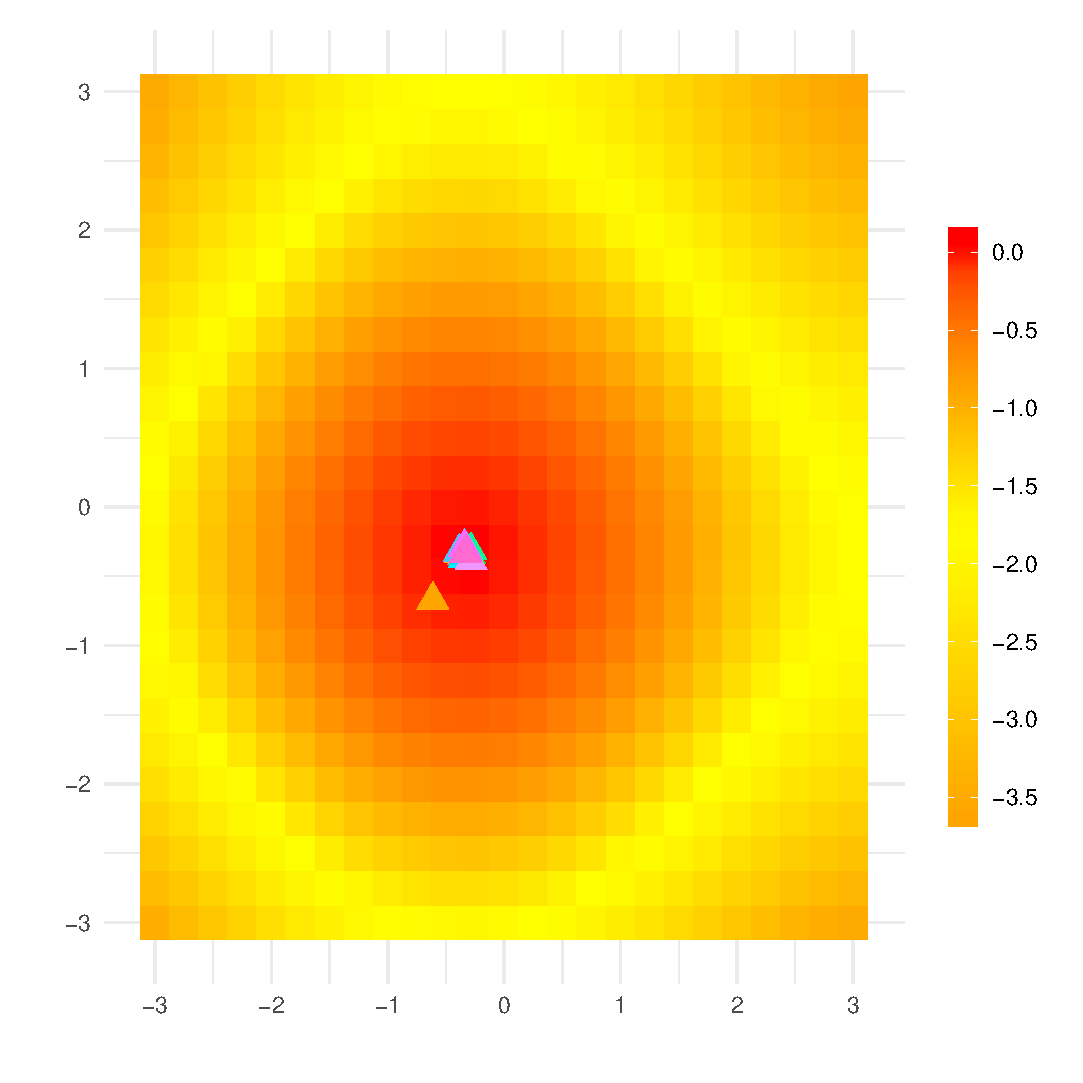
\includegraphics[width=60mm]{paso100.eps}}
 \subfloat[Busqueda local de m\'aximos en una proyecci\'on plana $(x,y)$, con 1000 pasos.]{
   \label{fig:paso1000}
    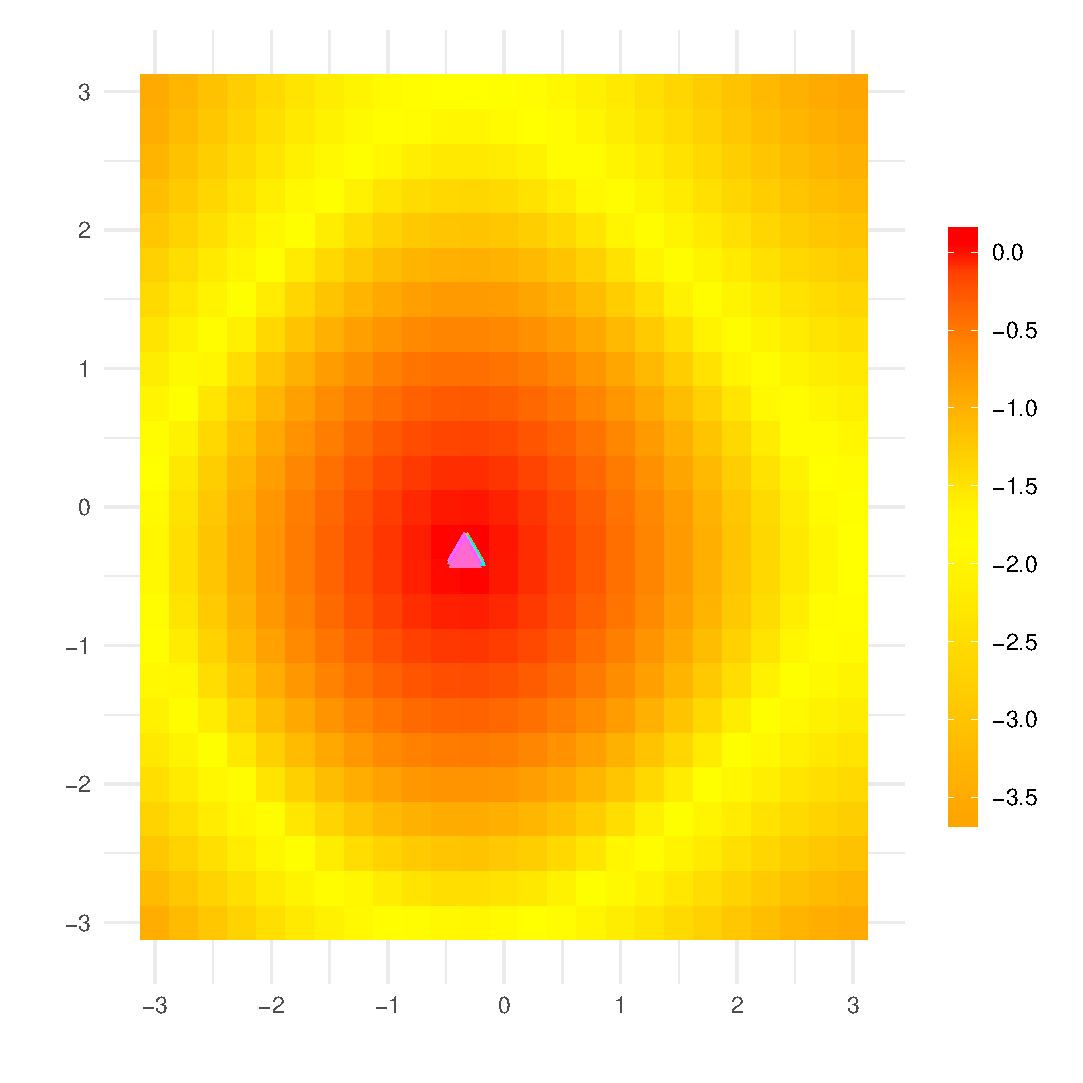
\includegraphics[width=60mm]{paso1000.eps}}
  \subfloat[Busqueda local de m\'aximos en una proyecci\'on plana $(x,y)$, con 10000 pasos.]{
   \label{fig:paso10000}
    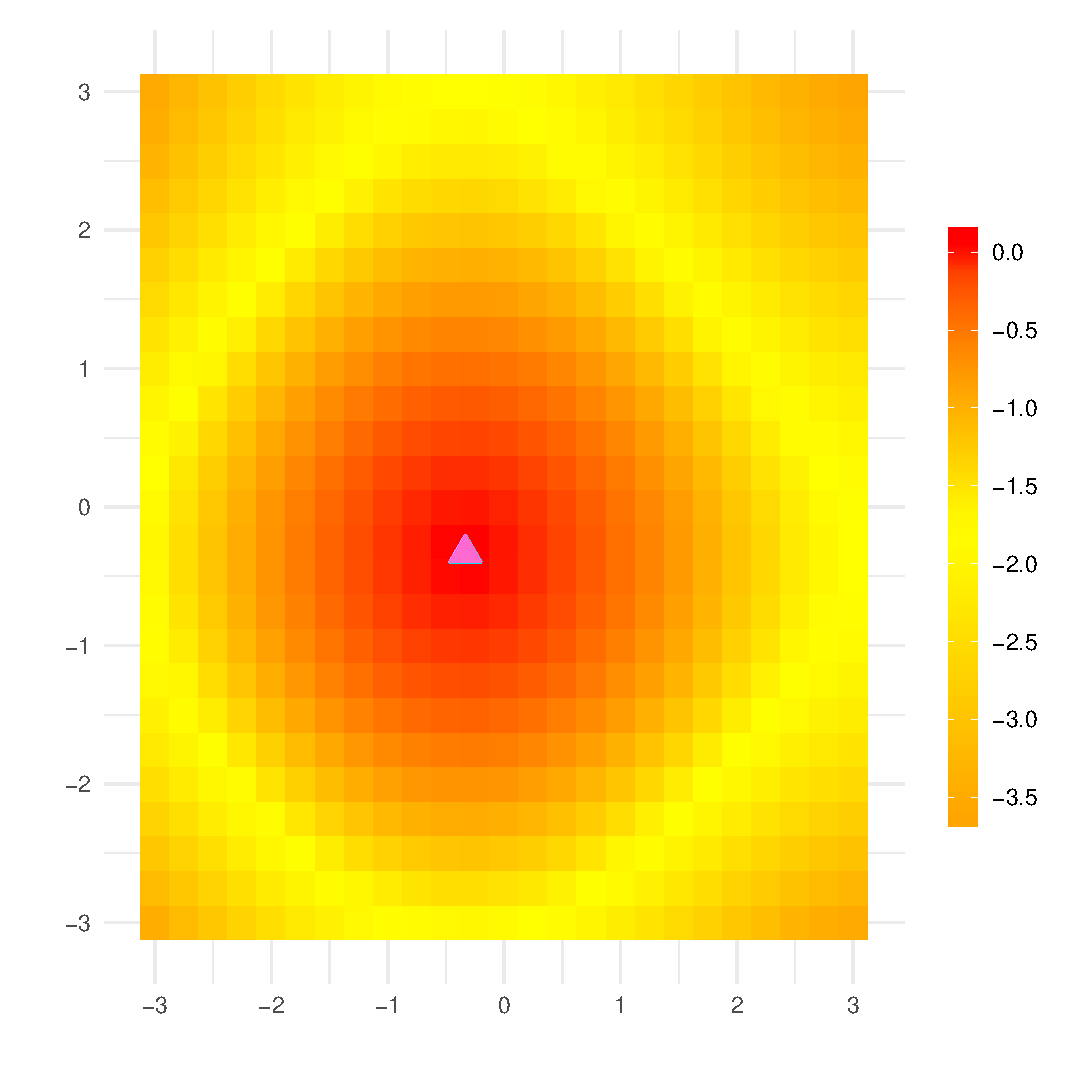
\includegraphics[width=60mm]{paso10000.eps}}
 \caption{Comparaci\'on de las r\'eplicas a mayor cantidad de pasos.}
 \label{fig:comparacion}
\end{figure}

Se obtuvo un \texttt{gif} ("busqueda\_animacion.gif") donde muestra el movimiento de cada r\'eplica en un per\'iodo de 100 pasos, localizado en el repositorio donde se encuentra esta pr\'actica \cite{repo}.

En la figura \ref{fig:comparacion}, tomando en cuenta que lo naranja indica los m\'inimos de la funci\'on $g(x,y)$ y lo rojo el m\'aximo, se observa que con 100 pasos la mayor\'ia de las r\'eplicas logra acercarse al m\'aximo de la funci\'on, cuando se realizan 10,000 pasos casi todas las r\'eplicas coinciden en el punto m\'aximo.

\newpage

\bibliographystyle{plainnat}
\bibliography{Bibliografias}
\end{document}